\chapter{Question 4}
\label{question-4}
\section{Question}

\begin{itemize}
\item Choose a news-related event
\item Use twarc.py to collect 1000 tweets, every day for 5 different days
	\begin{itemize}
	\item See: \url{https://github.com/edsu/twarc}
	\end{itemize}
\item For each day:
	\begin{itemize}
		\item Create a wall
		\item Build a tag/word cloud for each day
		\item Create a map using GeoJSON \& Github
		\begin{itemize}
			\item \url{https://help.github.com/articles/mapping-geojson-files-on-github/}
		\end{itemize}
	\end{itemize}
\item Discuss in detail lessons learned, experiences, etc.
\end{itemize}


\section{Solution}
\begin{itemize}
\item I chose `Google Fi' as the topic for this question.
\item I installed the twarc package using `sudo pip install twarc' on my ubuntu virtual machine.
\item I created a script to fetch 1000 tweets and ran this script for five consecutive days.
\item At the end of each day I followed the instructions of the author of the library to create the wall, word cloud, GeoJSON.
\item As I progressed to fetch the tweets for the fourth day I noticed it took longer to fetch tweets. I suspected this could be attributed to the reduction in the discussion about this topic.
\item Some of the tools provided by twarc are powerful.
\item The wall displays the tweets as a html which I didn't think was of much help as there are multitude of websites that provide this facility of displaying tweets based on search parameters.
\item I felt that the word cloud utility was a powerful feature that illustrates the words used in the tweet and the size of the word changes based on the frequency of usage in each of the tweets.
\item The geojson utility would be a good tool to visualize the contributors and their location if the geo-location is shared along with the tweet. But due to the limited tweets that had the co-ordinates it would be too premature to make more sense of the feature.
\item The html page generated by the wall utility is a good example of a file which would be boilerpipe successful. It has body content which can be extracted.
\item The html page generated by the wordcloud utility is a perfect example of a file which would not be boilerpipe successful because it has no body content but receives all its data through scripts.
\item I committed the files on github and the GeoJSON can be viewed using github pages from the following URL \url{https://github.com/maxbizarre/cs851-s15/blob/master/assignment4/twarc/tweetDay1.geojson} and \url{https://github.com/maxbizarre/cs851-s15/blob/master/assignment4/twarc/tweetDay2.geojson}.
\end{itemize}

	\begin{minipage}{\linewidth}
		\centering
			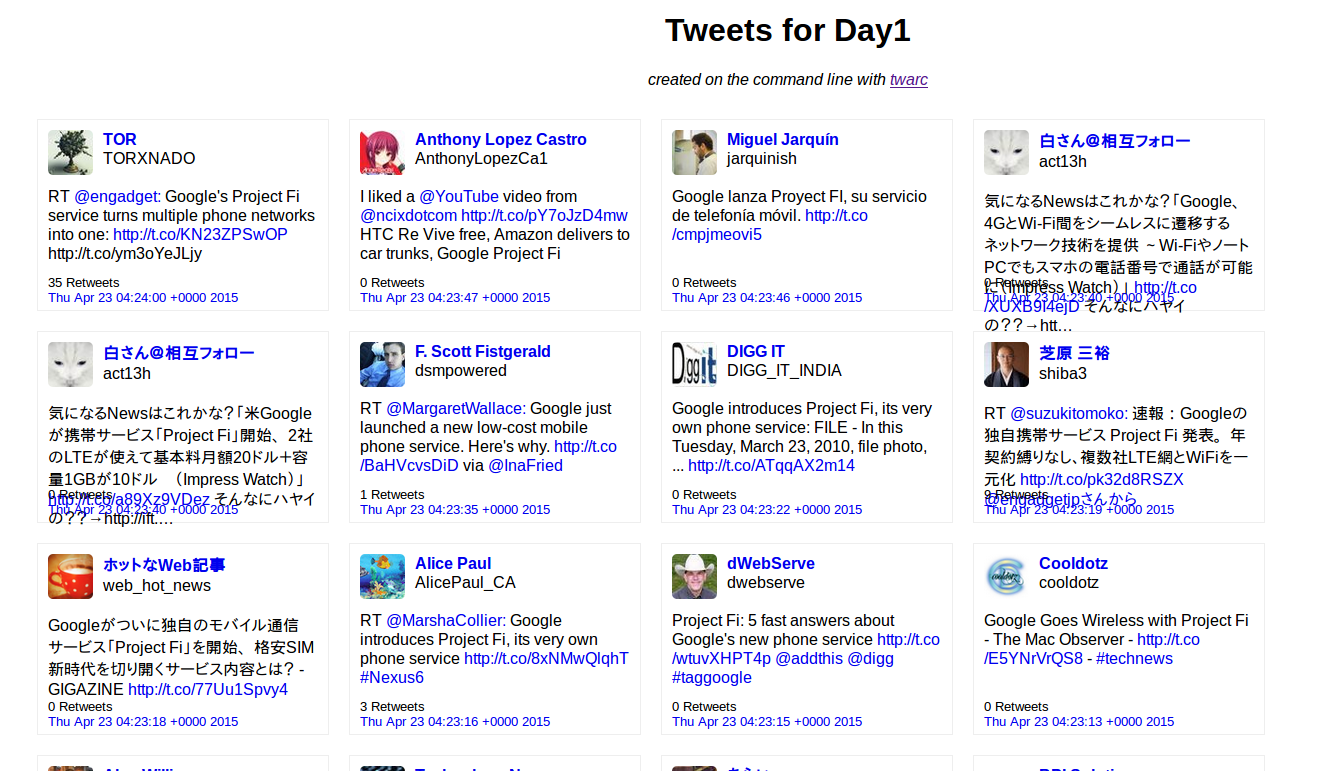
\includegraphics[scale=0.35]{figures/q4/wallDay1}
		\captionof{figure}{Wall - Day 1}
		\label{wordCount}
	\end{minipage}
	
	\begin{minipage}{\linewidth}
		\centering
			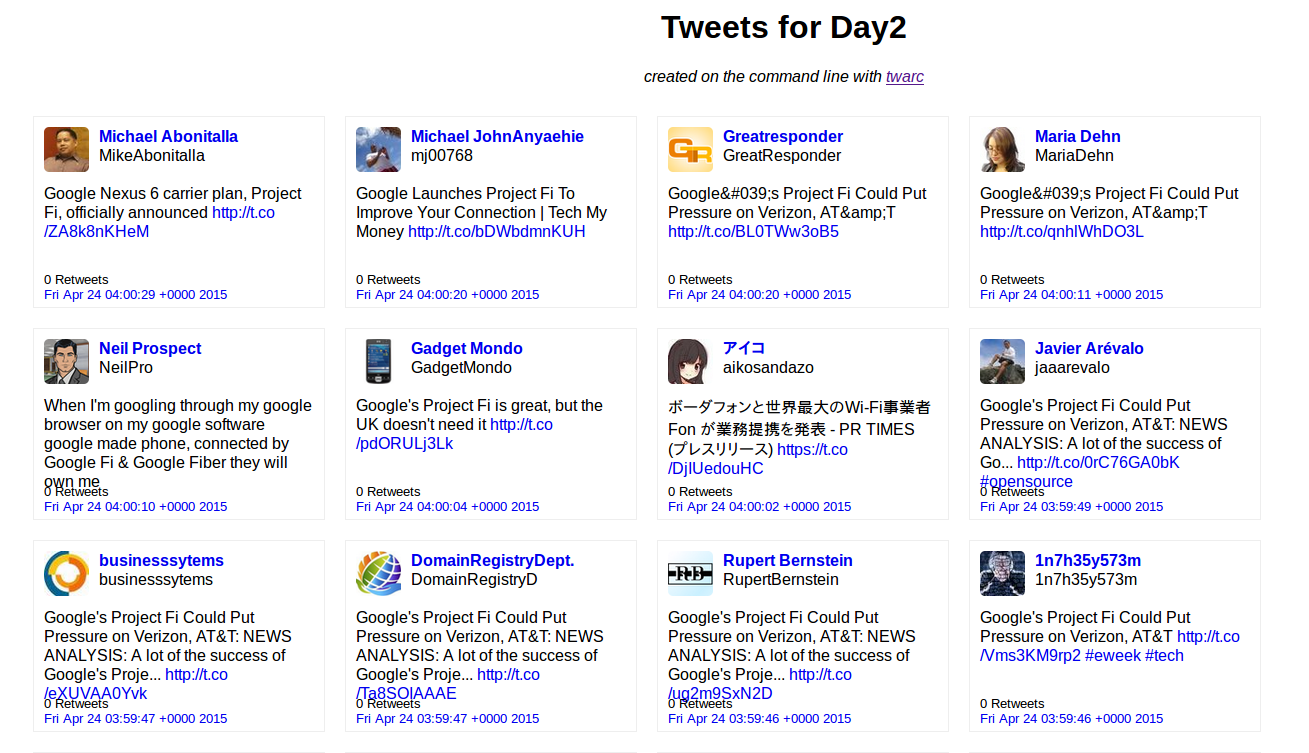
\includegraphics[scale=0.35]{figures/q4/wallDay2}
		\captionof{figure}{Wall - Day 2}
		\label{wordCount}
	\end{minipage}
	
	\begin{minipage}{\linewidth}
		\centering
			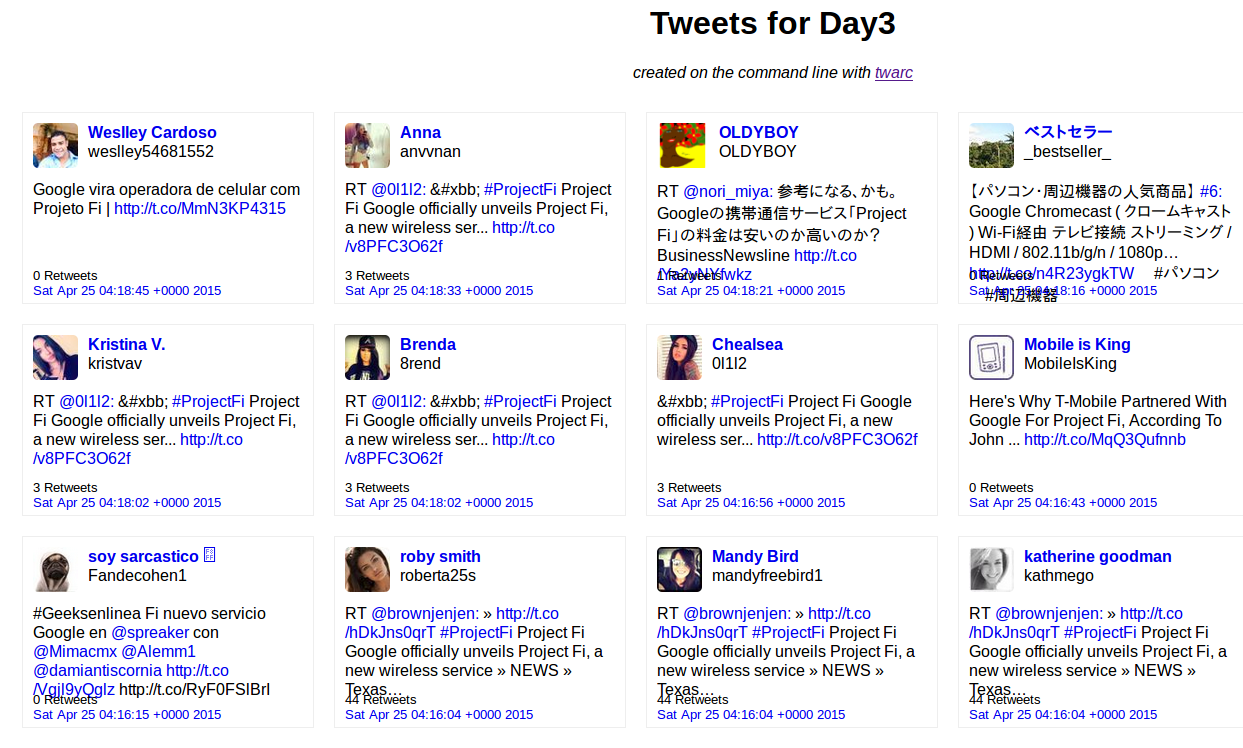
\includegraphics[scale=0.35]{figures/q4/wallDay3}
		\captionof{figure}{Wall - Day 3}
		\label{wordCount}
	\end{minipage}
	
	\begin{minipage}{\linewidth}
		\centering
			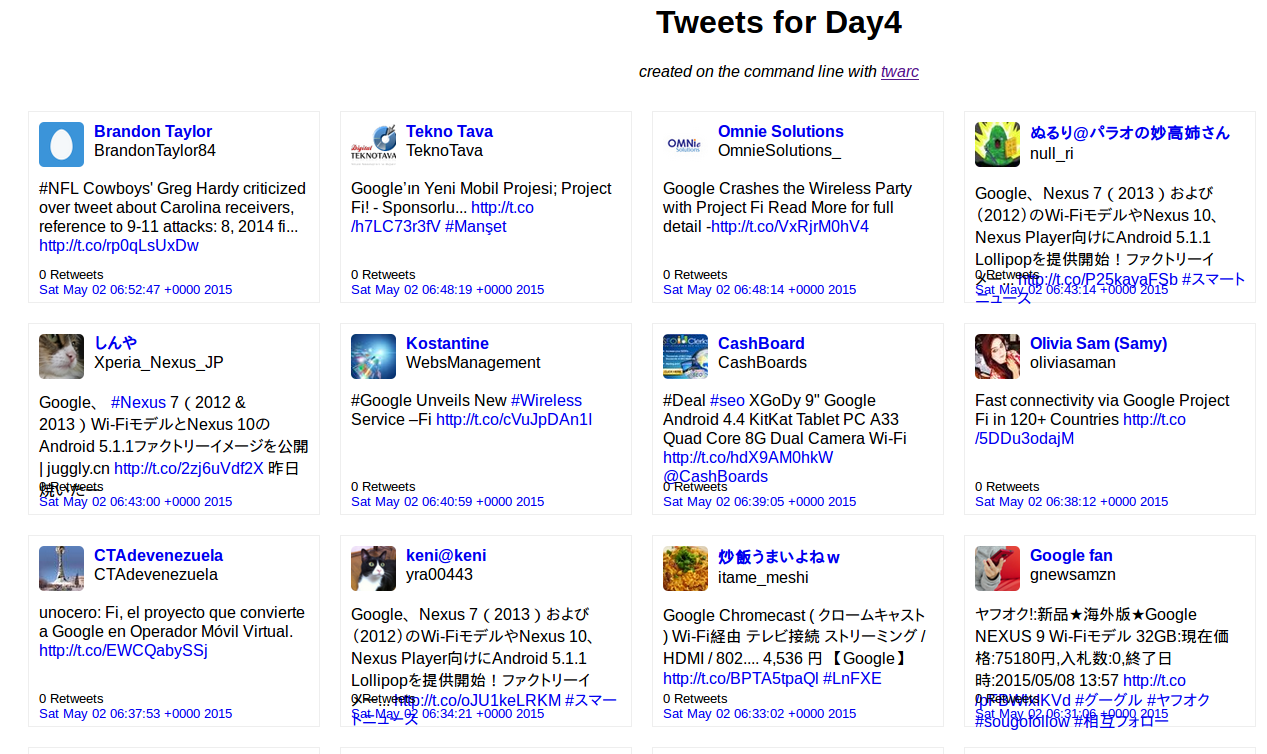
\includegraphics[scale=0.35]{figures/q4/wallDay4}
		\captionof{figure}{Wall - Day 4}
		\label{wordCount}
	\end{minipage}
	
	\begin{minipage}{\linewidth}
		\centering
			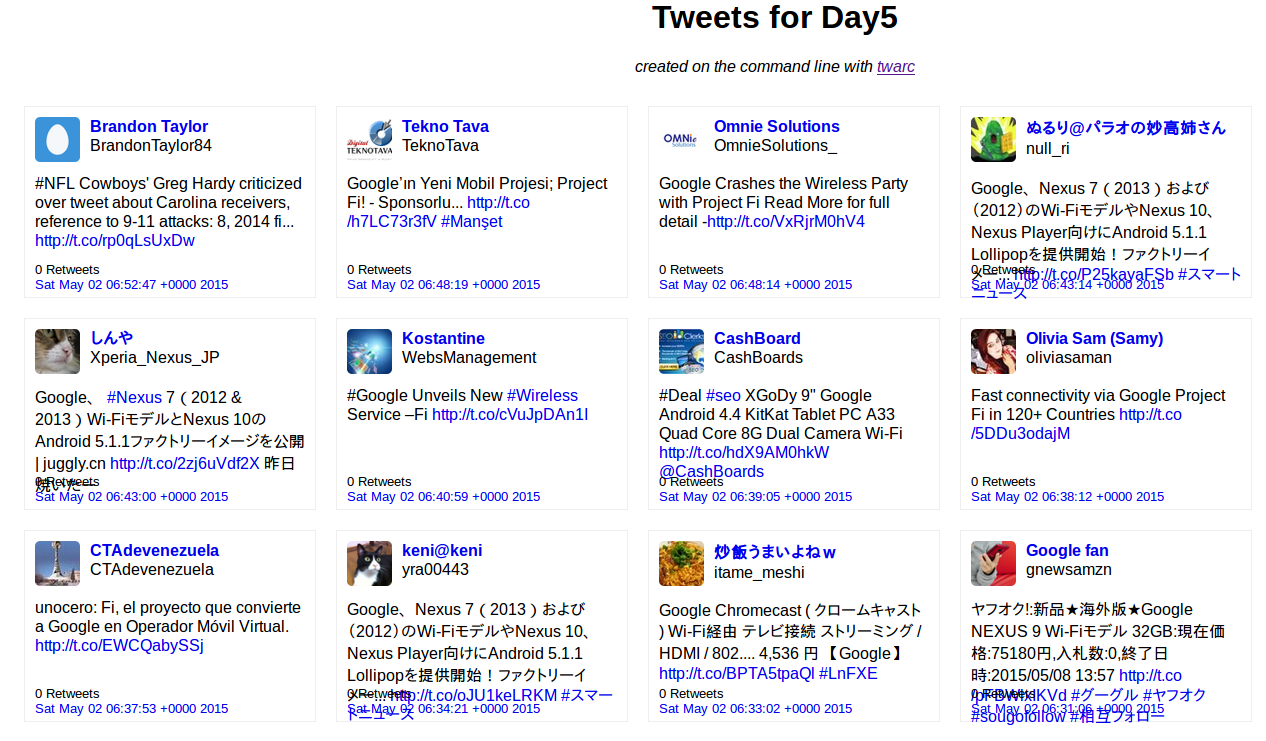
\includegraphics[scale=0.35]{figures/q4/wallDay5}
		\captionof{figure}{Wall - Day 5}
		\label{wordCount}
	\end{minipage}
	
	\begin{minipage}{\linewidth}
		\centering
			
\includegraphics[scale=0.55]{figures/q4/wordCloudDay1}
		\captionof{figure}{Word Cloud - Day 1}
		\label{wordCount}
	\end{minipage}
	
	\begin{minipage}{\linewidth}
		\centering
			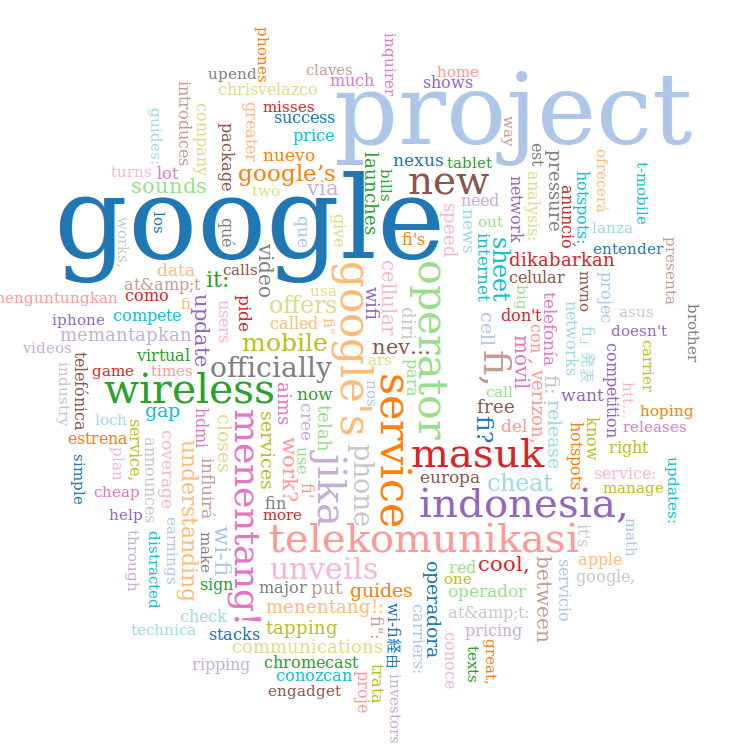
\includegraphics[scale=0.55]{figures/q4/wordCloudDay2}
		\captionof{figure}{Word Cloud - Day 2}
		\label{wordCount}
	\end{minipage}
	
	\begin{minipage}{\linewidth}
		\centering
			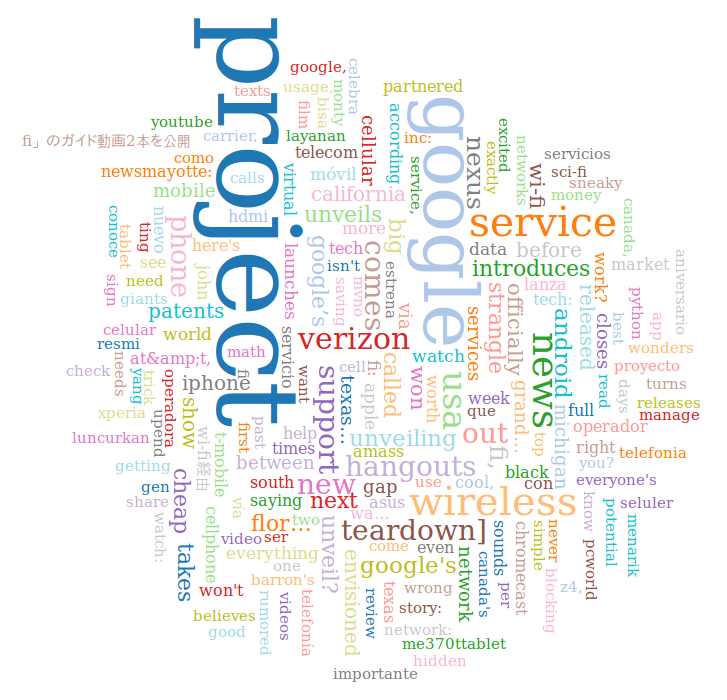
\includegraphics[scale=0.55]{figures/q4/wordCloudDay3}
		\captionof{figure}{Word Cloud - Day 3}
		\label{wordCount}
	\end{minipage}
	
	\begin{minipage}{\linewidth}
		\centering
			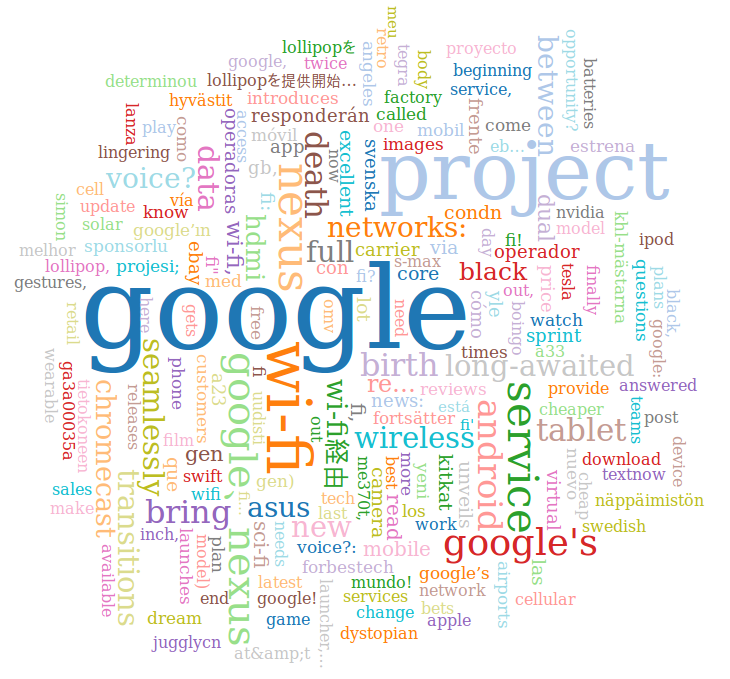
\includegraphics[scale=0.55]{figures/q4/wordCloudDay4}
		\captionof{figure}{Word Cloud - Day 4}
		\label{wordCount}
	\end{minipage}

	\begin{minipage}{\linewidth}
		\centering
			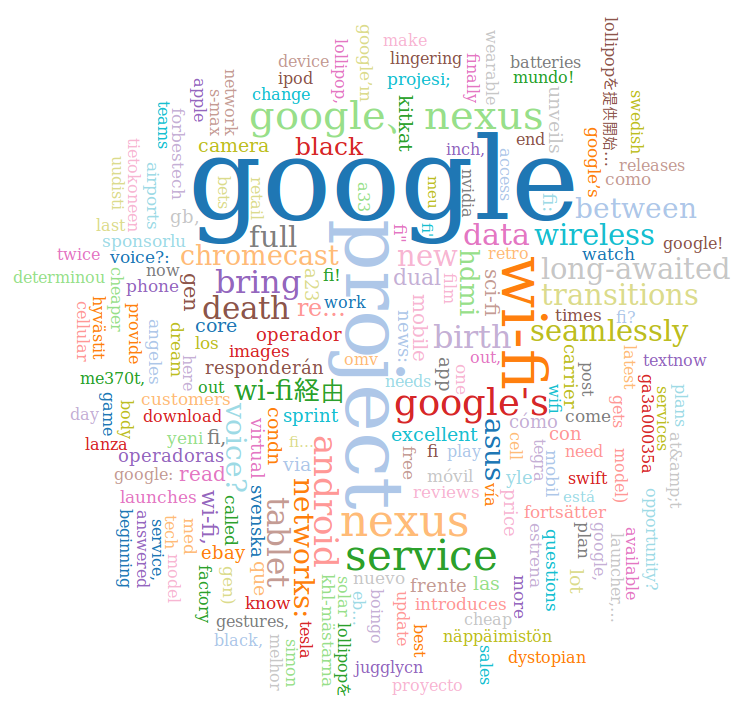
\includegraphics[scale=0.55]{figures/q4/wordCloudDay5}
		\captionof{figure}{Word Cloud - Day 5}
		\label{wordCount}
	\end{minipage}	
	
	\begin{minipage}{\linewidth}
		\centering
			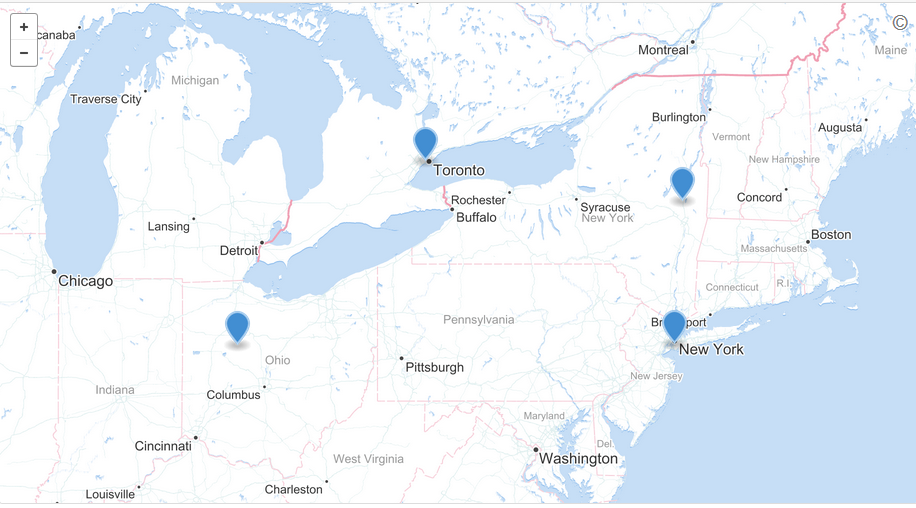
\includegraphics[scale=0.55]{figures/q4/geojsonDay1}
		\captionof{figure}{Geographical Location - Day 1}
		\label{wordCount}
	\end{minipage}

	\begin{minipage}{\linewidth}
		\centering
			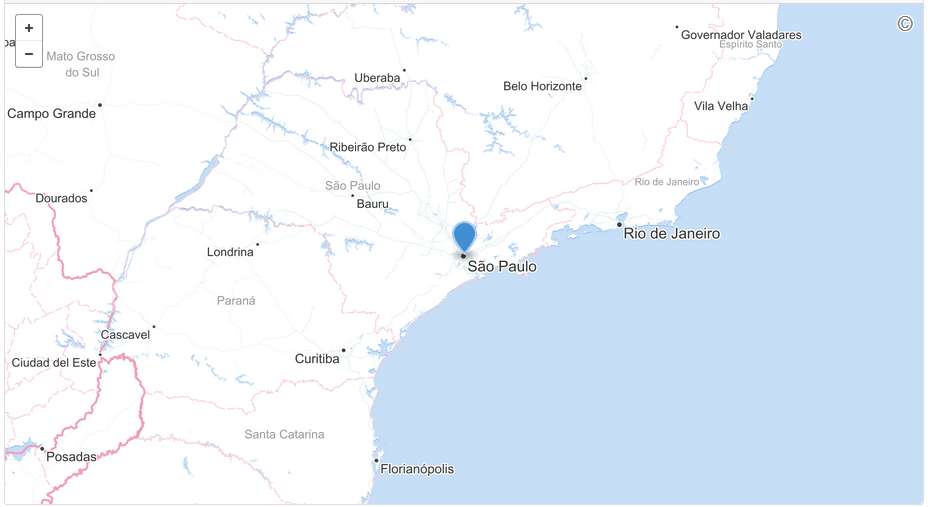
\includegraphics[scale=0.55]{figures/q4/geojsonDay2}
		\captionof{figure}{Geographical Location - Day 2}
		\label{wordCount}
	\end{minipage}	

\newpage
\section{Code Listing}

\lstinputlisting[language=Python,breaklines = true,frame=single,caption={Python program for fetching tweets using twarc.},label=lst:q1-1,captionpos=b,numbers=left,showspaces=false,showstringspaces=false,basicstyle=\footnotesize]{pythonFiles/getTweetTwarc.py}